\section{Overview pyramid}

\subsection{On what metrics does the system scores well or bad. How does it impact quality attributes ?}

\begin{itemize}
    \item ANDC too high -> high coupling, adding features more difficult, maintenance, subclass coupling
    \item AHH too high -> takes more time to compute (overloading) + \^ TO MUCH INHERITANCE
    \item NOM/NOC -> see below + small project -> not many methods -> ++ maintenance extensible
    \item LOC/NOM -> few methods per class but many lines per method => shoud refactor to have more modular methods -- maintenance extensible
    \item CYCLO/LOC -> flat code -> good because less tests -> mainly adding/storing data -> declarative language ??? ++ maintenance extensible
    \item CALL/NOM -> high but low FANOUT/CALL denotes that mostly operations from same class are called. so good coupling ++ maintenance extensible
    \item FANOUT/CALL -> low coupling thanks to facades ++ maintenance extensible
\end{itemize}

scores well on CYCLO NOM FANOUT

\subsection{How is each metric computed ?}

\begin{itemize}
    \item ANDC : average number of derived classes
    \item AHH : average hierarchy height
    \item NOM/NOC : number of methods / class
    \item LOC/NOM : number of lines of code / method
    \item CYCLO/LOC : proportion of lines of codes that are conditional branchement
    \item FANOUT : number of classes called in operations
    \item CALL : number of operations called from other operations (only one is counted per operation)
\end{itemize}

\subsection{Screenshots}

\begin{figure}[H]
    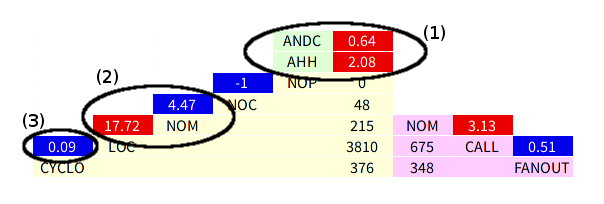
\includegraphics[width=\textwidth]{OverviewPyramid_annotated.png}
    \caption{\label{fig:pyramid}Overview pyramid with emphasis on important points}
\end{figure}

\begin{enumerate}
    \item Hierarchy is too big in both width and height. It denotes a strong coupling. The same features could probably be reached without inheritance
    \item Number of methods is good because it is not high but number of lines of code is too high. This could be fixed by splitting methods into smaller ones.
    \item Not many conditional branchements is very good for testing (both unit tests and integration tests) and to read and understand the code.
\end{enumerate}

\section{System attraction}
On the figure below, classes are represented as big black dots, methods as red dots and attributes as blue dots. The lines show the use of class methods and attributes by other classes and methods. In order to obtain this diagram in Moose, we choose the category \textbf{All model classes}, then select \texttt{Visulaize > System attraction}

\begin{figure}[H]
    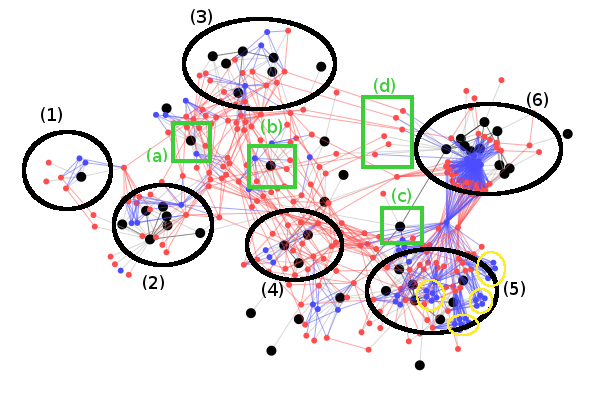
\includegraphics[width=\textwidth]{Attraction_annotated.png}
    \caption{\label{fig:attraction} Attraction diagram}
\end{figure}

\paragraph*{}
\begin{minipage}{0.6\textwidth}
  \begin{enumerate}
    \item InternetFrontend
    \item Pages (\begin{scriptsize}\texttt{LoginPage, QueryPage, ...}\end{scriptsize})
    \item Managers (\begin{scriptsize}\texttt{UserManager, ApplicationManager, ...}\end{scriptsize})
    \item Databases (\begin{scriptsize}\texttt{RawDatabase, RegularDatabase}\end{scriptsize})
    \item Database entries (\begin{scriptsize}\texttt{Book, Article, ...}\end{scriptsize})
    \item Registrations (\begin{scriptsize}\texttt{Administrator, CheapSubscription, ...}\end{scriptsize})
  \end{enumerate}
\end{minipage}\hfill
\begin{minipage}{0.3\textwidth}
  \begin{enumerate}[label=\alph*]
    \item ApplicationFacade
    \item DatabaseFacade
    \item Data
    \item UserProfile accessors
  \end{enumerate}
\end{minipage}

\paragraph*{}\textit{The other classes are not relevant for a complex system analysis (unit tests for instance).}

At first sight, this diagram looks like a spider web, with a few recognizable clusters of classes. The overall project does not seem to be well organized, because classes of different concerns seem to be linked together. The 3-tier architecture is not well implemented, otherwise we would clearly see the 3 layers on the visualization. Let's take a closer look.

\subsection{Users}
The cluster \texttt{(6)} contains the User classes, which are tightly grouped together. This indicates that they are highly coupled, because of their common ancestor: \texttt{Registration}. Interestingly enough, all of these classes are only used through a few attributes accessors (cluster \texttt{(d)} and right of cluster \texttt{(c)}), which means that they are loosely coupled to the rest of the system.

\subsection{Facades}
The \texttt{ApplicationFacade} (cluster \texttt{(a)}) and the \texttt{DatabaseFacade} (cluster \texttt{(b)}) do not fulfill their roles. A lot of links bypass them, which indicates that users of the facades are aware of what should be hidden behind the facade. In the ideal case, we should only see those classes as articulation nodes between clusters on the diagram.

\subsection{Data}
The data classes (cluster \texttt{(5)}) are also clearly identifiable. They are mostly accessed through the databases (cluster \texttt{(4)}). We attribute the \textit{spider web} feeling around the cluster to the tests cases (below cluster \texttt{(4)}). These data classes are essentially models (high number of attributes, few methods) as it can be seen in the small yellow clusters.

\section{Custom system complexity}
